\section{Statistical Formulas}
\label{stats:formulas}
The following mathematical expressions have been used for the statistical analysis.

\textbf{\large{Variance of the noise}}

\[
\hat{\sigma}^2 = \frac{1}{m-n} \mathbf{r}' \mathbf{r}
\]

Where $\mathbf{r}$ is the residuals vector, and $m$, $n$ are the dimensions of the matrix $A$.


\textbf{\large{Dispersion matrix of the parameters}}

\[
\mathbf{\Sigma} = \sigma \mathbf{(A' A)^{-1}}
\]

And $\sigma$ is the standard deviation of the noise.


\textbf{\large{Confidence interval of the parameters}}

\[
\hat{x}_i \pm t(m-n)_{1-\alpha / 2} \sigma (\mathbf{(A' A)^{-1}}_{ii})^{1/2} 
\]

Where $\hat{x}_i$ is the parameter estimation, $t(m-n)_{1-\alpha / 2}$ is the t-student with $m - n$ degrees of freedom and $\mathbf{(A' A)^{-1}}_{ii}$ is the corresponding value in the diagonal.


\textbf{\large{Confidence interval of the predictions}}
  
\[
\hat{y}_i \pm t(m-n)_{1-\alpha / 2} \sigma (\mathbf{a_i(A' A)^{-1}_{ii}a_i})^{1/2} 
\]

With $\hat{y}_i$ and $\mathbf{a_i}$ being the predicted value and the corresponding row in the matrix $\mathbf{A}$ respectively.


\textbf{\large{Prediction interval}}
  
\[
\hat{y}_i \pm t(m-n)_{1-\alpha / 2} \sigma (1+\mathbf{a_i(A' A)^{-1}_{ii}a_i})^{1/2} 
\]

As explained before, we see that the interval includes both the uncertainty of the expected value and the deviation of the data. 

\newpage
\section{Prediction Interval}
\label{pred:interval}


The figure below is an example of the $95 \%$ prediction interval for the least squares estimation mentioned in section 1.2. We see that the interval is wider than the corresponding confidence interval of the predictions.

\begin{figure}[htb]
\centering
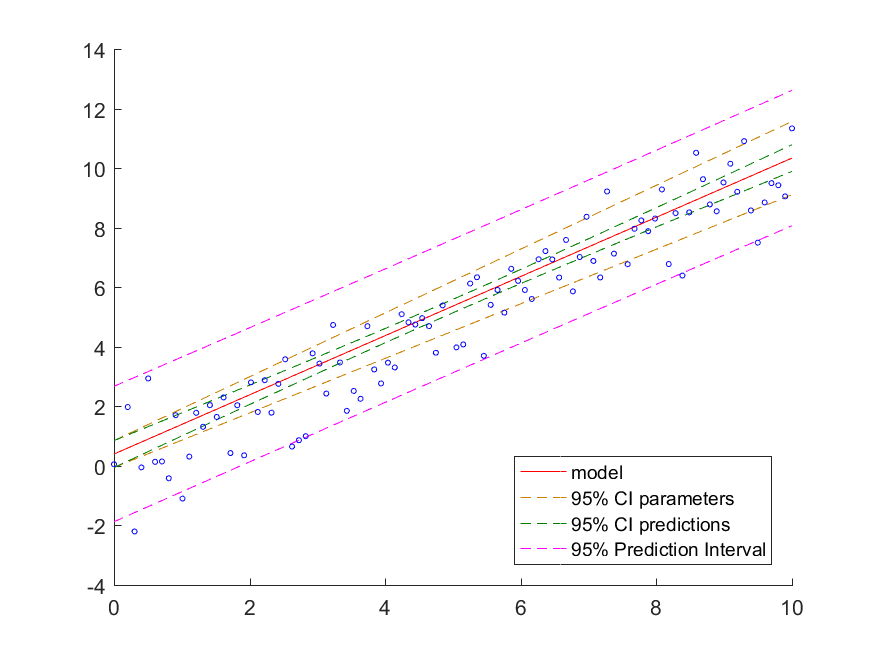
\includegraphics[width=0.7\textwidth]{../img/L2_Predic}
\caption{$L_2$ Prediction interval}
\label{fig:L2PI}
\end{figure}

\newpage
\section{Code for Part 1} 
\label{code:part1}
\subsection{L1\_norm.m}
\lstinputlisting[inputencoding=latin1]{"../Part\space 1/L1_norm.m"}

\newpage
\subsection{L2\_norm.m}
\lstinputlisting[inputencoding=latin1]{"../Part\space 1/L2_norm.m"}

\newpage
\subsection{Linfinity\_norm.m}
\lstinputlisting[inputencoding=latin1]{"../Part\space 1/Linfinity_norm.m"}

\newpage
\subsection{Huber.m}
\lstinputlisting[inputencoding=latin1]{"../Part\space 1/Huber.m"}

\subsection{dataPlot.m}
\lstinputlisting[inputencoding=latin1]{"../Part\space 1/dataPlot.m"}

\newpage
\subsection{stats.m}
\lstinputlisting[inputencoding=latin1]{"../Part\space 1/stats.m"}


\newpage
\section{Code for Part 2} \label{code:part2}
\subsection{main.m}
\lstinputlisting[inputencoding=latin1]{../Part2/main.m}

\subsection{michaelisMenten.m}
\lstinputlisting[inputencoding=latin1]{../Part2/michaelisMenten.m}

\newpage
\subsection{phiContours.m}
\lstinputlisting[inputencoding=latin1]{../Part2/phiContours.m}

\subsection{findStats.m}
\lstinputlisting[inputencoding=latin1]{../Part2/findStats.m}

\newpage
\subsection{phiContours2.m}
\lstinputlisting[inputencoding=latin1]{../Part2/phiContours2.m}

\subsection{findStats2.m}
\lstinputlisting[inputencoding=latin1]{../Part2/findStats2.m}

\newpage
\subsection{residuals.m}
\lstinputlisting[inputencoding=latin1]{../Part2/residuals.m}

\subsection{estimateY.m}
\lstinputlisting[inputencoding=latin1]{../Part2/estimateY.m}

\subsection{ModelAndSensitivity.m}
\lstinputlisting[inputencoding=latin1]{../Part2/ModelAndSensitivity.m}

\subsection{Derivatives.m}
\lstinputlisting[inputencoding=latin1]{../Part2/Derivatives.m}